\documentclass[12pt,a4paper]{report}

\renewcommand{\familydefault}{\sfdefault}

\usepackage[pdftex]{graphicx}
\usepackage{float}
\usepackage{fancyvrb}
\usepackage{minted}
\usepackage[utf8]{inputenc}
\usepackage[portuges]{babel}
\usepackage[T1]{fontenc}
\usepackage{times}
\usepackage[left=30mm,right=25mm,top=30mm,bottom=25mm,headsep=1.3cm]{geometry}
\usepackage{titlesec}
\usepackage{mathtools}
\usepackage{indentfirst}
\usepackage{rotating}
\usepackage{tabulary}
\usepackage{lscape}
\usepackage{enumerate}
\usepackage{amsfonts}
\usepackage{fancyhdr}
\usepackage{amsfonts}
\usepackage{tabu}
\usepackage{multicol}
\usepackage[table,xcdraw]{xcolor}
\usepackage{subfigure}
\usepackage{url}
\usepackage{hyperref}
\usepackage{enumitem}
\titlespacing*{\chapter}{0pt}{-0pt}{30pt}

\fancypagestyle{plain}{}
\pagestyle{fancy}
\fancyhead[L]{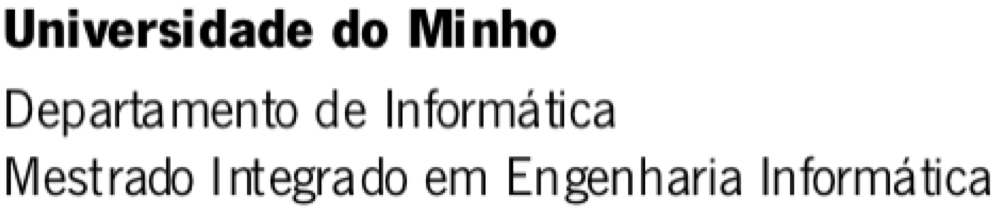
\includegraphics[scale=0.3]{Imagens/logoPB.png}}
\fancyhead[R]{Diagnóstico de um Projeto Ágil}

\AtBeginEnvironment{minted}{\fontsize{11}{11}\selectfont}

\newcommand{\HRule}{\rule{\linewidth}{0.5mm}}
\titleformat{\chapter}{\bfseries\huge}{\thechapter.}{20pt}{\huge}


\begin{document}

\nocite{*}
\begin{titlepage}

\newgeometry{left=5cm,top=0cm}

\begin{minipage}{0.6\textwidth}
\begin{flushleft} 

\includegraphics[width=\textwidth]{./Imagens/logo.png}
\end{flushleft}
\end{minipage}

\vspace{3cm}

\Huge

\textbf{Diagnóstico de um Projeto Ágil}

\LARGE

Gestão de Processo de Software 

\vfill

\normalsize

\textbf{Grupo de trabalho:}

Rogério Gomes Lopes Moreira, A74634

Samuel Gonçalves Ferreira, A76507

\vspace{5mm}

\textbf{Docente:}

Pedro Miguel Gonzalez Abreu Ribeiro


\vfill

Braga, {\today}

\end{titlepage}

\restoregeometry

\tableofcontents

\chapter{Introdução}

Redes neuronais artificias apresentam-se como um sistema conexionista, fortemente inspirado nas características do sistema nervoso central do ser humano. 
Apesar das RNAs serem um modelo simplificado, a sua arquitetura extremamente interligada de unidades de processamento permite que estas sejam capazes de generalizar e adquirir conhecimento, através de um processo de aprendizagem. 

Tirando partidos das suas características, vários algoritmos de \textit{Machine Learning} recaem sobre estas estruturas de aprendizagem, devido às suas capacidades de classificação e previsão em qualquer um dos paradigmas de aprendizagem. 

Neste projeto procura-se assim recorrer às capacidades de uma RNA, criada e modelada ao contexto do problema, para realizar a classificação do nível emocional de publicações da rede social \textit{Twitter}. 

No sentido de introduzir e uniformizar os conceitos em torno das RNAs, o presente relatório fornece inicialmente um descrição teórica dos principais temas associados com a modelação de uma rede neuronal artificial. 
Posteriormente, são descritas todas as etapas desenvolvidas ao longo do projeto e as decisões tomadas no decorrer deste.

Como estrutura do presente documento: o capítulo \ref{chp:rna} apresenta uma descrição breve daquilo que atualmente se entende por uma rede neuronal artificial, focando com relevo as características das suas unidades de processamento (neurónios), as arquiteturas existentes e o algoritmo de aprendizagem de \textit{Back-Propagation}; o capítulo \ref{chp:AnaliseDados} apresenta uma descrição da fase de pré processamento dos dados, focando a eliminação de ruído, seleção da informação útil e criação de novos atributos.

De seguida, numa vertente mais prática, os capítulos \ref{chp:criacaoRNAs} e \ref{cht:analiseresultados} apresentam, respetivamente, todas as considerações no processo de desenvolvimento e análise de resultados, ao longo dos diferentes cenários de teste realizados. 

Por fim, o capítulo \ref{chp:conclusao} apresenta as conclusões relativamente ao projeto e o trabalho futuro. 

\vspace{5cm}




\chapter{Os Métodos Ágil}
\label{cht:stateoftheart}

\section{A filosofia Ágil}

A metodologia Ágil descreve um conjunto de valores e princípios pelos quais os produtos são desenvolvidos. Entre esses princípios destacam-se o desenvolvimento incremental e iterativo, desenvolvimento adaptativo em vez de perspetivo, timeboxing e comunicação presencial em tempo real.
A ideia básica por trás do desenvolvimento iterativo e incremental é desenvolver um produto através de ciclos repetidos (iterativos) e em pequenas porções de cada vez (incremental). Aproveitando o que foi aprendido no passado, o cliente e a equipa melhoram iterativamente o produto até que este esteja completo. Em cada iteração, são feitas modificações a diferentes componentes.


Os métodos tradicionais de desenvolvimento baseiam-se no pressuposto de que um esforço muito significativo na fase de planeamento ajuda a evitar problemas e más decisões, contudo este tipo de método tem-se vindo a revelar pouco eficiente devido à incerteza do contexto interno e externo do projeto. Alterações nos requisitos, soluções, tecnologia ou prioridades, não só implicam alterações ao trabalho futuro como implicam reformulações no trabalho realizado.
\\
\begin{figure}[H]
    \centering
    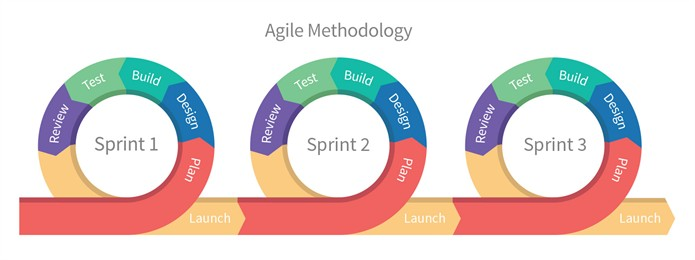
\includegraphics[scale=0.7]{Imagens/agil.jpg}
    \caption{Metodologia Ágil}
    \label{fig:agil}
\end{figure}
\\
Os métodos adaptativos, como os métodos Ágil, focam-se em reduzir o esforço inicial de planeamento e desenho da solução, colocando esse esforço no planeamento a curto prazo, mantendo apenas uma visão de alto nível a longo prazo. Quanto maior for o tempo de planeamento, mais vago é o planeamento desse período. Para além disso, o Ágil permite que o cliente possa alterar e avaliar o produto ao longo do desenvolvimento do mesmo, criando momentos onde o produto, o plano, as estimativas e abordagens possam ser avaliadas e melhoradas.


O timeboxing é usado como técnica de planeamento de projeto. A maioria dos métodos de desenvolvimento ágil partem o trabalho de desenvolvimento dos produtos em pequenos incrementos, minimizando a quantidade de planeamento. As iterações são períodos de tempo curto, também chamados de timeboxes. A cada iteração são selecionados requisitos para serem desenvolvidos nessa iteração, sendo que a restrição mais rígida é sempre o tempo.


Os métodos Ágil favorecem sempre a comunicação presencial, como forma de manter uma ligação próxima entre a equipa, o cliente e os restantes stakeholders. Ao contrário da comunicação escrita, a comunicação verbal em tempo real facilita a rápida e não constrangida troca de ideias, ajudando às boas relações e a criar um sentido de propriedade comum sobre o projeto.

Inicialmente os Métodos Ágil eram conhecidos como métodos leves. Em 2001 os membros da comunidade reuniram-se em Snowbird e adotaram o nome Métodos Ágil, tendo publicado o Manifesto Ágil, documento onde reúnem os princípios e práticas da metodologia de desenvolvimento. Mais tarde, foi formada a Agile Alliance, uma organização não lucrativa que promove o desenvolvimento Ágil. 
Alguns dos principais métodos Ágil incluem o Scrum, o Crystal Clear, a Programação extrema, o Adaptative Software Development, o Feature Driven Development e o Dynamic Systems Development Method.

\newpage

\section{Scrum}

Ken Schwaber, cofundador da metologia Scrum e um dos envolvidos na formação da Agile Alliance, define esta metodologia recordando um momento algo divertido:

\begin{quote}
Quando me perguntaram em que consistia o meu trabalho, respondi que ajudo pessoas a desenvolver software em 30 dias. E o sujeito olhou para mim e disse ”Então, não tenho de esperar 180 dias para ter aquilo que não quero? ”Sim, exatamente, nós damos-lhe aquilo que não quer em 30 dias.
\end{quote}

\begin{figure}[H]
    \centering
    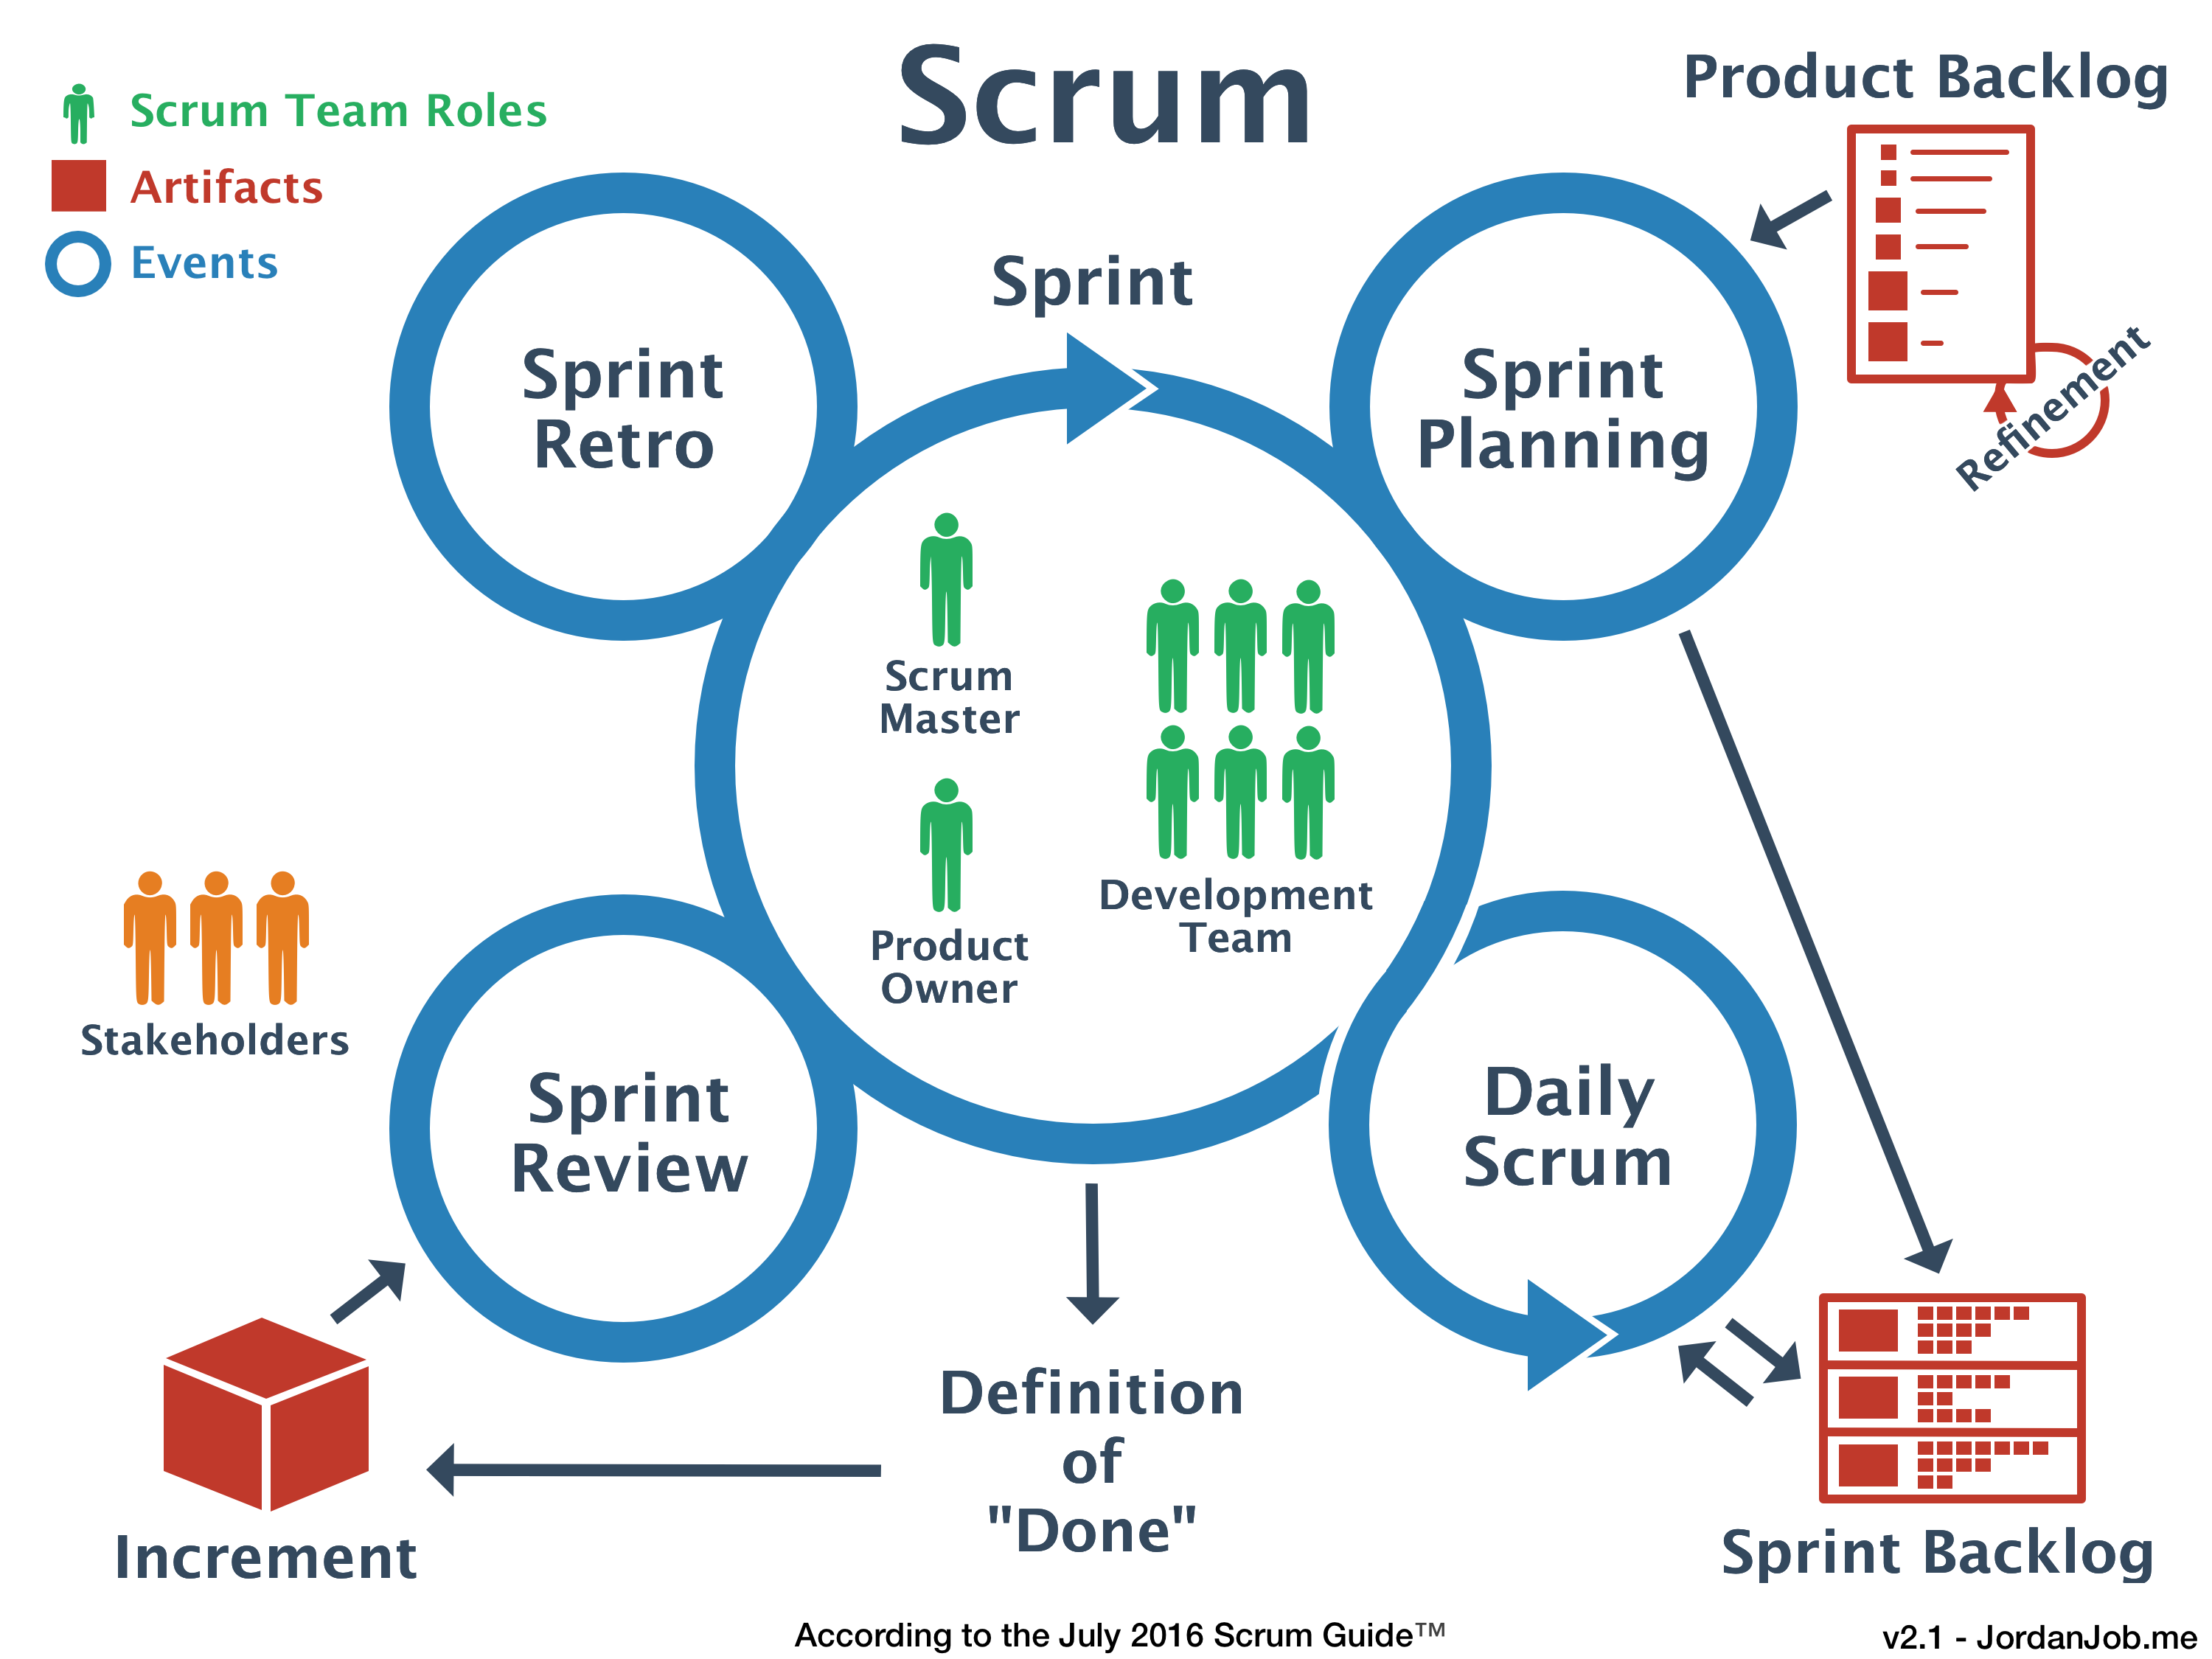
\includegraphics[scale=0.60]{Imagens/scrum.png}
    \caption{Metodologia Scrum}
    \label{fig:scrum}
\end{figure}

Assentando os seus princípios fundamentalmente em boas práticas de gestão, o Scrum assume-se como uma metodologia extremamente ágil e flexível. Tem por objetivo definir um processo iterativo e incremental de desenvolvimento de produtos ou gestão de projetos. Produz um conjunto de funcionalidades potencialmente mais próximas do objetivo final ao fim de cada iteração.
\\
Centrado no trabalho em equipa, melhora a comunicação e maximiza a cooperação permitindo que cada um faça o seu melhor, aumentando a produtividade. O método Scrum, pode-se aplicar a projetos grandes ou pequenos, esforçando-se para libertar o processo de quaisquer barreiras, o seu principal objetivo é conseguir uma avaliação correta do ambiente em evolução. Ao contrário do que se possa imaginar, embora o Scrum englobe processos de engenharia, este não requer nem fornece qualquer técnica ou método específico para o desenvolvimento do software, apenas estabelece um conjunto de regras e práticas de gestão.

\subsection{Como nasceu o conceito?}

A metodologia Scrum, desenvolvida por \textit{Ken Schwaber} e \textit{Jeff Sutherland} e inspirada nas ideias de desenvolvimento rápido e concorrente de produtos de \textit{Hirotaka Takeuchi} e \textit{Ikujiro Nonaka}, nasceu da necessidade de encontrar uma metodologia que abordasse o problema do desenvolvimento de software de uma forma não tradicional, em que a equipa age como um todo para atingir os seus objetivos.

Algumas datas importantes:

\begin{itemize}
\item 1993 - Ken Schwaber desenvolveu na ADM uma framework iterativa e incremental;
\item 1993 - Metodologia Scrum implementada pela primeira vez por uma equipa
liderada por Jeff Sutherland na Easel Corporation;
\item 1994 - Sutherland definiu o Scrum em Easel;
\item 1994 - Ken and Jeff refinam Scrum;
\item 1996 - IDX usa Scrum em projectos com aproximadamente 600 pessoas;
\item 1996 - Scrum é apresentado na OOPSLA (international conference on Object Oriented Programming Systems, Languages and Applications);
\item 2000 - Práticas ”eXtremme Programming”usadas conjuntamente com Scrum (XP @ Scrum);
\item 2001 - Ken Schwaber e Mike Beedle editam o primeiro livro de Scrum;
\item 2003 - Certificações Scrum;
\end{itemize}

\newpage

\subsection{Vocabulário Específico}

\begin{itemize}
    \item \textbf{Backlog} - Lista de todas as funcionalidades a serem desenvolvidas durante o projeto completo, sendo bem definido e detalhado no inicio do trabalho, deve ser listado e ordenado por prioridade de execução.
    \item \textbf{Sprint} - Período não superior a 30 dias, onde o projeto (ou apenas algumas   funcionalidades) é desenvolvido.
    
    \item \textbf{Sprint Backlog} - Trabalho a ser desenvolvido num Sprint de modo a criar um produto a apresentar ao cliente. Deve ser desenvolvido de forma incremental, relativa ao Backlog anterior (se existir).
    
    \item \textbf{Scrum Meeting} - Reunião diária onde são avaliados os progressos do projeto e as barreiras encontradas durante o desenvolvimento.
    
    \item \textbf{Scrum Rules} - Protocolo a seguir de modo a realizar uma reunião Scrum. 
    
    \item \textbf{Scrum Team} - Equipa de desenvolvimento de um Sprint.

    \item \textbf{Scrum Master} - Elemento da equipa responsável pela gestão do projeto e liderar os Scrum Meetings.
\end{itemize}

\subsection{Regras do Scrum}

É necessário respeitar algumas regras de execução, nomeadamente no que diz respeito aos Backlog, Sprint e Scrum Meetings.
\\
Relativamente ao BackLog, devem ser debatidos pela equipa todos os pontos que devem integrar a lista de funcionalidades da aplicação, sendo de responsabilidade do Scrum Master a ordenação da lista por prioridade de execução.
\\
Relativamente ao Sprint, deve ser realizado num período não superior a 30 dias e não deve ter uma equipa superior a 9 elementos. Devem além disso, ter um objetivo claro, baseado no BackLog e este não deve ser modificado enquanto o Sprint está a decorrer, à exceção de novas funcionalidades que, segundo o Scrum Master, tenham influência no decorrer do projeto e que possam ser completadas no Sprint. Caso o Sprint estiver a tomar um rumo não desejável, é possível dissolver o Sprint e começar um novo, com base no Sprint
Backlog.
\\
Os Scrum Meetings são um ponto de grande importância no desenvolvimento de um projeto. É nas reuniões que o Scrum Master deve atualizar-se do decorrer do projeto e procurar identificar os pontos de conflito do desenvolvimento, podem agir para os eliminar. Estas reuniões devem ser diárias, sempre à emsma hora e no mesmo local, com duração não superior a 30 minutos. Toda a conversa deve ser restringida às perguntas colocadas pelo Scrum Master, sendo elas:

\begin{enumerate}
    \item O que foi desenvolvido desde a última reunião?
    \item Que dificuldades foram encontradas durante o desenvolvimento?
    \item O que está planeado para ser desenvolvido até à próxima reunião?
\end{enumerate}

Todos os elementos devem responder às perguntas anteriores e com base nelas o Scrum Master deve tomar as decisões por forma a remover todas as situações que impeçam o bom decorrer do desenvolvimento do projeto.

\subsection{O processo}

Para se dar início ao processo de Scrum, o primeiro passo é decidir a constituição da equipa para trabalhar. Esta equipa não deve ter mais de 6 a 9 membros. Se houver mais membros do que o possível gerir, separam-se várias equipas Scrum e cada equipa focar-se-á em áreas específica do projeto.
\\
A próxima coisa a afazer é apontar o Scrum Master, uma vez que é essa pessoa que conduz os Scrum Meetings, medindo o progresso e tomando as decisões necessárias para remover os obstáculos encontrados.
\\
É vital para que o processo funcione cumprir com os trabalhos rigorosamente com base nos pontos restantes do Sprint Backlog. Para isso é preciso estabelecer e conduzir reuniões diárias Scrum onde as equipas encontram e atualizam o seu estado atual. Isto fornece um foco diário no trabalho em desenvolvimento.

\begin{figure}[H]
    \centering
    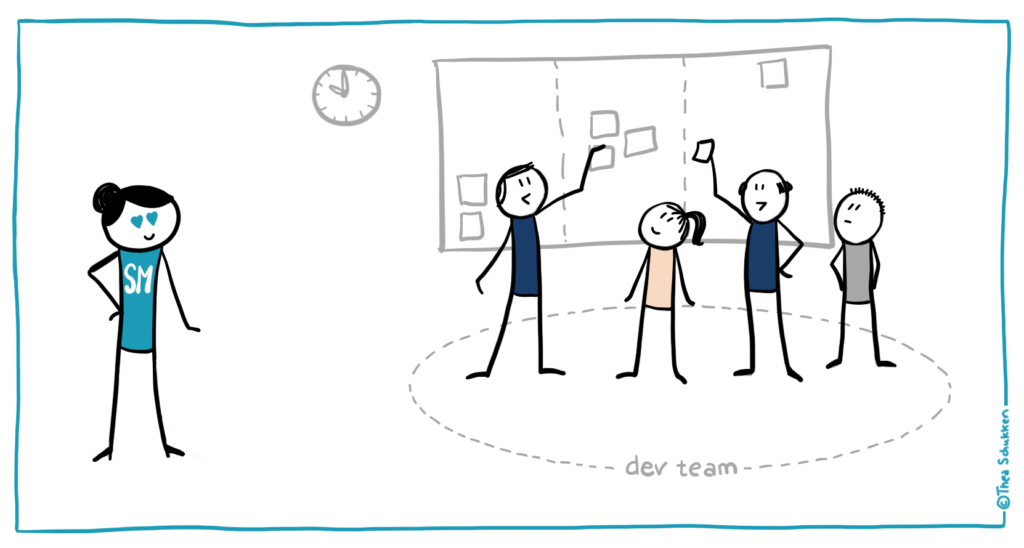
\includegraphics[scale=0.4]{Imagens/team.png}
    \caption{Equipa Scrum}
    \label{fig:equipascrum}
\end{figure}

\newpage

\section{Kanban}

Kanban é um termo de origem japonesa e significa literalmente “cartão” ou “sinalização”. Este é um conceito relacionado com a utilização de cartões (post-it e outros) para indicar o andamento dos fluxos de produção sendo que em cada cartão é colocada informação sobre uma determinada tarefa. Os cartões são depois organizados em listas que representam o processo de desenvolvimento do produto. Um exemplo de organização de listas é “Por fazer”, “Em progresso” e “Concluído”. À medida que o trabalho progride, a equipa vai movendo os cartões entre as diferentes secções.

\begin{figure}[H]
    \centering
    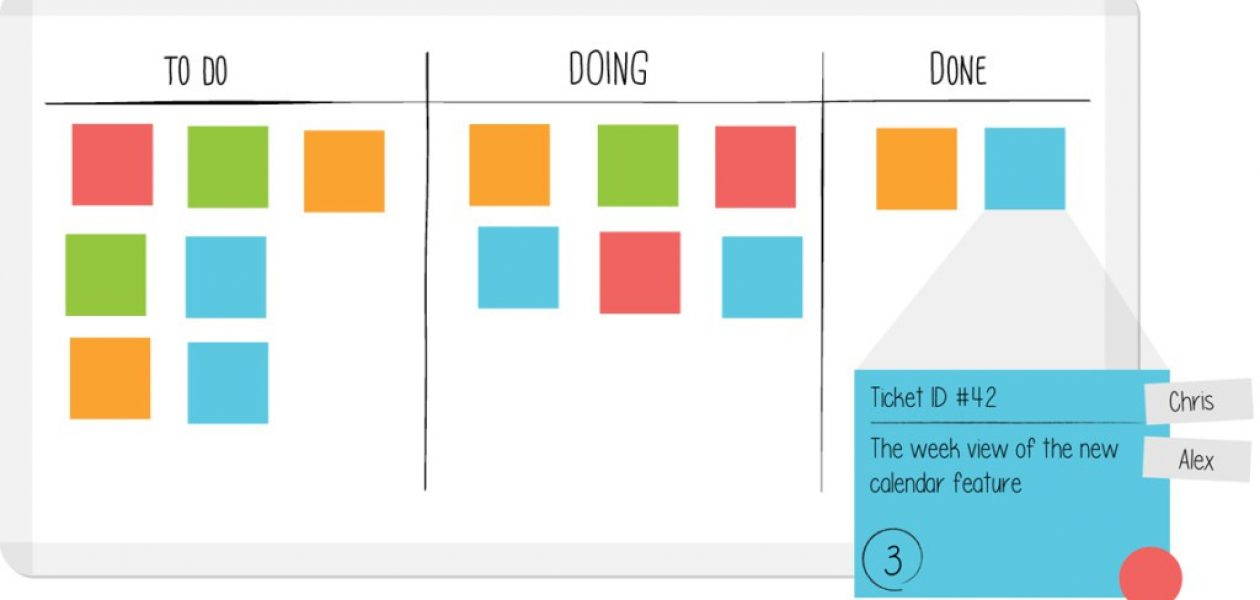
\includegraphics[scale=0.3]{Imagens/kanban.jpg}
    \caption{Quadro Kanban}
    \label{fig:equipascrum}
\end{figure}

\subsection{Como nasceu o conceito?}

Nos finais de 1940, a \textit{Toyota} começou a otimizar os seus processos baseando-se no mesmo modelo que os supermercados usavam para dispôr stock nas prateleiras. Os supermercados adquirem apenas as quantias necessárias de produtos para servir a procura dos consumidores, uma prática que otimiza o fluxo entre o supermercado e o consumidor. Como os níveis de inventário seguem os padrões de consumo, o supermercado ganha eficiência significativa na gestão de inventário ao diminuir o excesso de stock possuído a qualquer momento. Mesmo assim, o supermercado consegue garantir que um determinado produto que um consumidor precisa vai estar sempre em stock.

Quando a \textit{Toyota} aplicou este sistema, o objetivo era alinhar melhor os seus níveis enormes de stock com o consumo real de materiais. Para comunicar níveis de capacidade em tempo real na fábrica (e aos fornecedores), os trabalhadores passavam um cartão, ou "kanban", entre as equipas. Quando um contentor de materiais usados na linha de produção era esvaziado, um kanban era passado para o depósito, descrevendo o material do qual se precisava, a sua quantia exata e assim em diante. O depósito contava com um novo contentor desse material em espera, o qual era enviado para a fábrica que, por sua vez, enviava o seu próprio kanban para o fornecedor. O fornecedor também tinha um contentor com esse material em espera, o qual seria enviado para o depósito. Embora a tecnologia de sinalização desse processo tenha evoluído desde a década de 1940, esse mesmo processo de fabricação "just in time" (ou JIT) continua no centro do processo.

\subsection{Vocabulário Específico}

\begin{itemize}
    \item \textbf{Just in Time (JIT)} - Sistema de administração da produção que determina que tudo deve ser produzido, transportado ou comprado na hora exata.
    
    \item \textbf{Kanban de Produção} - Cartão que autoriza a produção de determinada quantidade de um item.
    
    \item \textbf{Kanban de Movimentação (ou Kanban de Transporte)} - Cartão que autoriza a movimentação física de peças entre o processo do fornecedor e o processo do cliente (se houver).
    
\end{itemize}

\subsection{O processo}

Para pôr o Kanban em prática (em particular na produção de Software), deve-se começar por definir quais os estados possíveis de uma tarefa ("por fazer", "em desenvolvimento", "feito"...). Depois de bem definidos os estados, deve-se usar uma ferramenta de suporte à representação destes estados que irão conter listas de tarefas. Para isto pode-se usar um quadro, uma folha de cálculo, uma ferramenta de gestão de tarefas (p.ex: Trello) ou qualquer outro método que sirva este propósito.

De seguida devem ser listadas as tarefas destinadas a ser desenvolvidas num determinado período de tempo e estas devem ser colocadas sob o grupo "por fazer". A partir daqui, sempre que alguém começar uma determinada tarefa deve imediatamente mudar o estado da tarefa para "em desenvolvimento" de maneira a que todos os restantes elementos da equipa saibam que alguém já começou a trabalhar nessa tarefa.

Quando se termina uma tarefa, esta deve imediatamente ser mudada para o próximo estado no fluxo definido inicialmente. Neste caso, pode ser logo considerada resolvida, pode estar sujeita a revisão ou pode ainda ter que ser alvo de testes unitários, o que significa que existiria uma tarefa associada a ela que consistiria em desenvolver os testes para essa tarefa.

O Kanban costuma ser aliado ao Scrum ou a outras metodologias, visto que o Kanban por si só não define limites temporais para cada tarefa ou conjunto de tarefas.

\newpage

\section{Extreme Programming (XP)}

Extreme Programming, é uma metodologia ágil para equipas pequenas e médias que desenvolvem software com requisitos vagos e em constante mudança. Para isso, adota a estratégia de constante acompanhamento e realização de vários pequenos ajustes durante o desenvolvimento de software.

Os cinco valores fundamentais da metodologia XP são: comunicação, simplicidade, feedback, coragem e respeito. A partir destes valores, tem como princípios básicos: feedback rápido, presumir simplicidade, mudanças incrementais, aceitar mudanças e trabalho de qualidade.

Dentre as variáveis de controlo em projetos (custo, tempo, qualidade e escopo), há um foco explícito em escopo. Para isso, recomenda-se a priorização de funcionalidades que representem maior valor possível para o negócio. Desta forma, caso seja necessária a diminuição de escopo, as funcionalidades menos valiosas serão adiadas ou canceladas.
\begin{figure}[H]
    \centering
    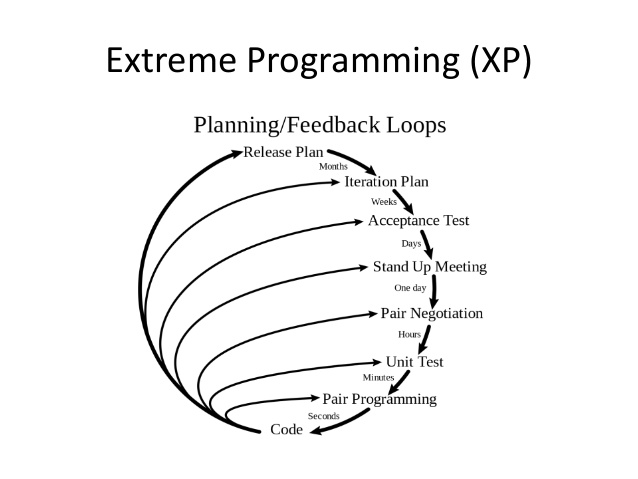
\includegraphics[scale=0.60]{Imagens/xp.jpg}
    \caption{Metodologia XP}
    \label{fig:scrum}
\end{figure}
A XP incentiva o controlo da qualidade como variável do projeto, pois o pequeno ganho de curto prazo na produtividade, ao diminuir qualidade, não é compensado por perdas (ou até impedimentos) a médio e longo prazo.


\subsection{Como nasceu o conceito?}
Extreme programming foi criada por Kent Beck durante o seu trabalho no projeto Chrysler Comprehensive Compensation System (C3). Beck tornou-se o líder do projeto C3 em março de 1996 e começou a refinar a metodologia de desenvolvimento usada no projeto.

Kent Beck foi convidado para o projeto C3 para aumentar a performance do sistema, mas o seu cargo aumentou à medida que ele foi reparando em vários problemas no processo de desenvolvimento. Beck aproveitou esta oportunidade para propôr e implementar algumas alterações nas práticas do C3 baseadas no seu trabalho com o seu frequente colaborador, Ward Cunningham. 

Beck convidou Ron Jeffries para o projeto para ajudar a desenvolver e refinar estes métodos. Depois disso Jeffries atuou como um treinador para incutir as práticas e hábitos na equipa do C3.

Os princípios e práticas por detrás do XP foram disseminadas pelo mundo através de discussões na wiki original, \textit{Cunningham's WikiWikiWeb}. Vários contribuidores discutiram e expandiram as ideias, e algumas metodologias resultaram.


\subsection{Valores do XP}
\begin{itemize}
    \item \textbf{Comunicação} – para um projeto de sucesso é necessária muita interação entre os membros da equipa, programadores, cliente, treinador. Para desenvolver um produto, a equipa precisa de ter muita qualidade nos canais de comunicação. Conversas cara-a-cara são sempre melhores do que telefonemas, e-mails, cartas ou fax.
    
    \item \textbf{Feedback} – as respostas às decisões tomadas devem ser rápidas e visíveis. Todos devem ter, a toda a hora, consciência do que está a acontecer.
    
    \item \textbf{Coragem} – alterar um código em produção, sem causar bugs, com agilidade, exige muita coragem e responsabilidade.
    
    \item \textbf{Simplicidade} – para atender rapidamente às necessidades do cliente, quase sempre um dos valores mais importantes é a simplicidade. Normalmente o que o cliente quer é muito mais simples do que aquilo que os programadores constroem. 
    \item \textbf{Respeito} – todos têm sua importância dentro da equipa e devem ser respeitados e valorizados.

\end{itemize}

\subsection{Papéis do XP}
\begin{itemize}
    \item \textbf{Programadores} – foco central da metodologia, sem hierarquia.
    
    \item \textbf{Treinador (ou coach)} – pessoa com mais experiência na equipa, responsável por lembrar os outros das regras do jogo (que são as práticas e os valores de XP). O treinador não precisa necessariamente ser o melhor programador da equipa e sim o que mais entende da metodologia XP.
    
    \item \textbf{Acompanhador (ou tracker)} – responsável por trazer para a equipa dados, gráficos, informações que mostrem o andamento do projeto e ajudem a equipa a tomar decisões de implementação, arquitetura e design. Algumas vezes o próprio coach faz papel de tracker. Outras vezes a equipa escolhe quem exercerá este papel.
    
    \item \textbf{Cliente} – em XP o cliente faz parte da equipa. Deve estar sempre presente e pronto para responder às dúvidas dos programadores.

\end{itemize}

\subsection{Práticas do XP}
\begin{itemize}
    \item \textbf{Planeamento} – assim como no Scrum, existe uma fase de planeamento, quando os desenvolvedores e cliente se encontram para priorizar e estimar histórias.
    
    \item \textbf{Fases Pequenas} – cada fase é chamada de iteração (Sprint no Scrum). Cada fase deve durar no máximo 30 dias, mas o ideal é que seja 15 ou até 7 dias.
    
    \item \textbf{Design Simples} – seguindo o valor simplicidade, os projetos devem ser simples e atender em cada passo apenas o que foi pedido.
    
    \item \textbf{Testes} – todo o desenvolvimento de software inclui testes. Kent Beck diz que código sem testes não existe. Os testes devem ser escritos de preferência antes do desenvolvimento (TDD – test driven development) e devem ser sempre executados de forma automatizada.
    
    \item \textbf{Refatoração} – é um conjunto de técnicas para modificar o código do sistema sem alterar nenhuma funcionalidade. O objetivo é simplificar, melhorar o design, limpar, deixar o código mais fácil de entender e dar manutenção.
    
    \item \textbf{Programação em pares} – em XP dois programadores sentam-se no mesmo computador e programam juntos. Enquanto um programador escreve, o outro observa e pensa em melhorias e alternativas.
    
    \item \textbf{Propriedade Coletiva} – O código fonte não pertence a um único programador. Todos da equipa são responsáveis. Todos alteram código de todos.
    
    \item \textbf{Integração Contínua} – depois de testada, cada nova funcionalidade deve ser imediatamente sincronizada entre todos os programadores. Quanto mais frequente for essa integração, menores são as hipóteses de conflitos de ficheiros que vários programadores alteram simultaneamente.
    
    \item \textbf{Semana de 40 horas} – programar é uma atividade intensa e que não rende se o programador não estiver descansado e disposto. Por isso, 40 horas de trabalho por semana é essencial para a saúde da equipa.
    
    \item \textbf{Cliente Sempre Presente} – o cliente não é alguém de fora, mas sim um membro da equipa. Ele deve estar sempre disponível e pronto para atender às dúvidas dos programadores.
    
    \item \textbf{Padronizações} – se toda a equipa seguir padrões pré-acordados de programação, será mais fácil manter e entender o que já está feito. O uso de padrões é uma das formas de reforçar o valor comunicação.
\end{itemize}


\newpage

\section{Dynamic Systems Development Method (DSDM)}

A DSDM (Dynamic Systems Development Methodology) é uma metodologia Ágil de apoio ao desenvolvimento de software. O principal foco desta metodologia é o desenvolvimento de uma aplicação com a qualidade desejada sem ultrapassar os limites temporais e orçamentais. Para isto, o método DSDM tem em consideração a interação com o cliente e o utilizador final, entregando protótipos frequentemente, tendo equipas de desenvolvimento autónomas, testes durante todo o processo e uma lista de requisitos priorizada. A DSDM fornece assim uma framework para uma abordagem interativa e incremental no desenvolvimento de Sistemas de Informação. Começou a ser desenvolvida nos anos 90 na Inglaterra e foi aplicada pela primeira vez em 1995. O DSDM é uma mistura de várias técnicas, surgindo como uma extensão do RAD (Rapid Application Development) e focado em projetos com prazos e orçamentos apertados.
A DSDM aborda os problemas que frequentemente ocorrem no desenvolvimento de informação que se prendem essencialmente com a falta de tempo, com orçamentos apertados ou outro tipo de razões para que o projeto falhe, tal como a falta de envolvimento dos encarregados do projeto ou dos utilizadores finais. 

\subsection{Princípios da DSDM}

A DSDM apresenta alguns princípios chave. Estes princípios delimitam as bases do desenvolvimento utilizando DSDM. 

\begin{itemize}
    \item O ponto fundamental desta metodologia prende-se com a entrega de um sistema que se aproxime das necessidades do negócio. Não é uma metodologia tão direta que forneça todas as necessidades de negócio, mas centraliza todo o potencial na concretização final de todos os objetivos do projeto.
    \item Nenhum sistema é completamente construído na primeira tentativa. Num processo de desenvolvimento de um sistema informático 80\% da solução pode ser desenvolvida em 20\% do tempo necessário para encontrar a solução perfeita. Para aperfeiçoar a parte final poderá ser necessário que o projeto ultrapasse o seu tempo e orçamento estipulados. Uma vez que a DSDM é caracterizada por realizar exatamente o que a empresa necessita, é muitas vezes desnecessário chegar à solução perfeita.
    \item A entrega do projecto deve ser feita na data estipulada, dentro do orçamento previsto e com boa qualidade.
    \item As exigências para o Sistema de Informação têm que ser flexíveis. Tal como falaremos mais tarde, exigências flexíveis são tópicos importantes da DSDM.
    \item Esta metodologia apenas requer que cada etapa do desenvolvimento seja completada até que seja possível iniciar o passo seguinte. Isto faz com que cada fase do projeto possa começar sem ter que esperar que as fases que começaram anteriormente sejam totalmente terminadas.
    \item A comunicação entre todas as partes envolvidas (stakeholders) é também um pré-requisito bastante importante para que o projeto corra com a eficiência desejada.
    \item O envolvimento dos utilizadores é a chave para esta eficiência.
    \item As equipas responsáveis têm que ser dotadas de um sentido de decisão, sendo este também um ponto fulcral na progressão do projeto.
    \item Tal como as equipas de desenvolvimento também as equipas de gestão do projeto estão incorporadas na DSDM.
    \item Após o desenvolvimento do Sistema de Informação, a DSDM pode também ser usado para expandir o Sistema obtido.
\end{itemize}

\subsection{Fases do DSDM}

A framework DSDM consiste em três fases sequenciais: Pré-Projeto, Projeto e Pós-Projeto. A fase de Projeto do DSDM é a mais elaborada das três fases e consiste em 5 níveis formadas por uma abordagem passo-a-passo e iterativa no desenvolvimento de um SI.

\begin{figure}[H]
    \centering
    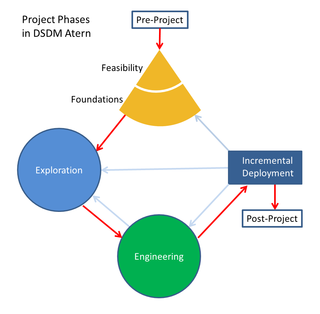
\includegraphics[scale=1]{Imagens/dsdm.png}
    \caption{Metodologia DSDM}
    \label{fig:dsdm}
\end{figure}

\subsubsection{Fase 1 - Pré-Projeto}

Na fase do pré-projeto, o projeto candidato é identificado, tratando-se depois do seu plano de financiamento e sendo assegurado um compromisso de realização. Tratar destas questões numa fase inicial evita problemas futuros em fases mais avançadas do desenvolvimento do projeto.

\subsubsection{Fase 2 - Projeto}

A visão geral de um processo DSDM, presente na Fig. 3, representa o Ciclo de Vida do Projeto nesta segunda fase da metodologia. Ela mostra os 5 níveis que a equipa de desenvolvimento terá de percorrer para criar um SI. Os dois primeiros níveis, o Estudo de Viabilidade e o Estudo de Negócio, são fases sequenciais que se complementam. Depois destas fases estarem concluídas, o sistema é desenvolvido iterativamente e de forma incremental nos níveis de Análise Funcional, Desenho e Implementação.

\subsubsection{Fase 3 - Pós-Projeto}

A fase de pós-projeto assegura um sistema de atuação eficiente. Isto é implementa- do através da manutenção e melhoramentos de acordo com os princípios da DSDM. Até mesmo a iniciação de novos projetos, para atualizar o sistema existente ou desenvolver um novo sistema, é possível.

\subsection{Principais Conceitos}

\begin{itemize}
    \item Timeboxing - É uma das técnicas utilizadas nos projec- tos baseados na metodologia DSDM. Esta técnica é utilizada para suportar um dos objetivos principais da DSDM: realizar o desenvolvimento de um Sistema de Infor- mação no tempo previsto, dentro do orçamento e com a qualidade desejada. A principal ideia por de trás do Timeboxing é dividir o projeto em porções, cada uma com um orçamento fixo e uma data de entrega estipulada. Para cada porção, é selecionado um número de requisitos que são escalonados de acordo com o princípio de MoSCoW. Uma vez que o tempo e o orçamento são fixos, a única variável restante é aquela que representa os requisitos. Portanto, se um projeto está a ficar sem tempo ou dinheiro, os requisitos com menor prioridade são omitidos. Isto significa, efectivamente, que um produto incompleto é entregue, devido aos princípios subjacentes à DSDM de que 80\% do projeto pode ser realizado em 20\% do tempo que leva a construir o produto completo e de que nenhum sistema é construído na perfeição à primeira tentativa.
    \item MoSCoW - A técnica MoSCoW representa um método de definição de prioridades nas tarefas efetuadas. Neste contexto, a técnica MoSCoW da DSDM é usada para dar prioridade aos requisitos enunciados. É um acrónimo que representa:
MUST have this.
SHOULD have this if at all possible.
COULD have this if it does not affect anything else. WON'T have this time but WOULD like in the future.
TEM de ter isto.
DEVE ter isto se for possível de todo.
PODE ter isto se não afetar o resto.
NÃO VAI ter isto agora mas SERIA bom ter no futuro.
    \item Prototipagem - Esta técnica refere-se à criação de protótipos do sistema em desenvolvimento numa fase inicial do projeto. Ela possibilita a descoberta antecipada de possíveis problemas no sistema e o teste por parte dos futuros utilizadores do sistema. Deste modo, é conseguido um bom envolvimento do utilizador final com o sistema, sendo este um dos principais fatores de sucesso da DSDM.
    \item Workshop - Esta é uma das técnicas de um projeto DSDM que tem como alvo juntar os diferentes stakeholders fazendo com que estes discutam as requisições estipuladas e as funcionalidades do produto, levando, no fim, a um entendimento mútuo. Num workshop, os stakeholders reúnem-se e discutem o projeto.
    \item Testes - Outro aspeto de relevo dos objetivos da DSDM é a criação de um SI com boa qualidade. Para obter esta solução, a DSDM obriga a efetuar testes em todas as iterações. Uma vez que a DSDM é uma metodologia independente de ferramentas e técnicas, a equipa do projeto é livre de escolher o seu próprio método de realização de testes.
    
\end{itemize}

\newpage

\section{Adaptive Software Development}


O Adaptive Software Development (ASD) é uma técnica criada especificamente para o desenvolvimento de sistemas de software complexos, proposta por Jim Highsmith em 2000. Este método Ágil apoia-se na colaboração humana e na auto-organização dos intervenientes no processo, aparecendo quando estes cooperam para criar resultados, que seriam impossíveis de criar individualmente.

\subsection{Fases do ASD}

O método ASD tem, à semelhança de outros métodos, três fases: Especulação, Colaboração e Aprendizagem.

\begin{figure}[H]
    \centering
    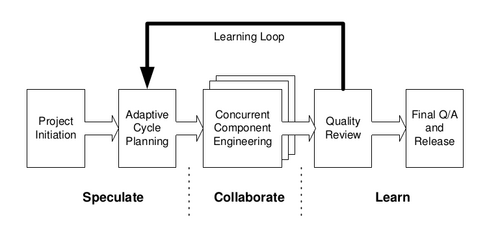
\includegraphics[scale=0.8]{Imagens/asd.png}
    \caption{Metodologia ASD}
    \label{fig:asd}
\end{figure}

\subsubsection{Fase 1 - Especulação}

Por vezes, o termo de planeamento é algo muito determinístico que indica um grau de certeza sobre o resultado desejado e que nem sempre é o caminho mais desejado para um determinado projeto de software, impedindo a equipa de levar o projeto para direções inovadoras e distintas do plano original.
No método ASD, o termo de planeamento é substituído pelo termo especulação. Ao especular, a equipa não abandona o plano, mas reconhece a realidade da incerteza em problemas de complexa resolução. Especular incentiva a exploração e a experimentação em ciclos iterativos curtos.

\subsubsection{Fase 2 - Colaboração}

Um dos princípios base do ASD é o facto das aplicações complexas não serem simplesmente construídas, mas sim que evoluem ao longo do tempo. As aplicações complexas exigem que um grande volume de informações sejam colecionado, analisado e aplicado ao problema, ou seja, é necessário uma colaboração intrínseca entre toda a equipa. Nesta fase é necessário gerir projeto com técnicas tradicionais e criar e manter o ambinete de colaboração.

\subsubsection{Fase 3 - Aprendizagem}

A fase da aprendizagem do ciclo é vital para o sucesso do projeto. A equipa precisa de aprimorar o seu conhecimento constantemente, usando para isso práticas como:

\begin{itemize}
    \item Revisões Técnicas
    \item Retrospetivas do projeto
    \item Grupos de foco com o cliente
\end{itemize}

As iterações precisam ser curtas, para que a equipe possa aprender com pequenos erros em vez de grandes.


\subsection{Principais Conceitos}

\begin{itemize}
    \item Mission Driven - Para cada iteração do ciclo de desenvolvimento justifica-se através de uma missão, que pode mudar ao longo do projeto.
    \item Component-Based - Desenvolvimento orientado a componentes, desenvolvendo o software em pequenas partes.
    \item Iterative - Desenvolvimento de pequenos ciclos (iterações), com o objetivo de resultar numa implementação satisfatória para cada missão definida por iteração. No ASD é melhor refazer do que fazer corretamente à primeira.
    \item Time Boxed - Fixação de prazos para evitar ambiguidade em projetos, com prazos tangíveis forçando a que a equipa defina decisões do projeto no início.
    \item Change-Tolerant - As mudanças são frequentes. É sempre melhor estar pronto a adaptar.
    \item Risk-Driven - Todos os pontos que são considerados características de alto risco são priorizados.
\end{itemize}

\newpage

\section{Crystal Methods}

Os Crystal Methods são uma família de metodologias de desenvolvimento de software e, como os cristais, possuem diferentes cores e rigidez, referindo-se ao tamanho e ao nível crítico do projeto.
Estes métodos foram originalmente desenvolvidos por Alistair Cockburn e Jim Highsmith com o objetivo de conseguir uma abordagem de desenvolvimento de software que premiasse a "manobrabilidade" durante o que Cockburn caracteriza como “um jogo de cooperação de invenções e comunicação de recursos limitados, com o principal objetivo de entregar softwares úteis a funcionar e com o objeto secundário de preparar-se para o jogo seguinte”.
Assim, os métodos Crystal são focados nos talentos e nas habilidades de cada pessoa, permitindo que o processo de desenvolvimento seja moldado conforme as características da equipa que o vai desenvolver, misturando a sua cultura de trabalho com a proposta de desenvolvimento Ágil.
As duas métricas envolvidas na adequação do projeto são: o número de pessoas envolvidas e o nível crítico do projeto.

\subsection{Métricas do Crystal}

Cada método Crystal é caracterizado por uma cor, de acordo com o número de envolvidos na equipa:


\begin{itemize}
    \item Crystal Clear é uma metodologia leve, para equipas de uma a oito pessoas, podendo chegar até doze em casos especiais;
    \item Yellow, para equipas por volta de dez a vinte membros;
    \item Orange e a variante Orange Web são apropriados para equipas de vinte a cinquenta participantes;
    \item Red para equipas de cinquenta a cem membros. Cada um dos métodos tem graus de gestão e de comunicação ajustados de acordo ao tamanho da equipa.
\end{itemize}

Além das cores, o Crystal utiliza algumas letras para representar potenciais perdas causados por uma falha no sistema de desenvolvimento de software.

\begin{figure}[H]
    \centering
    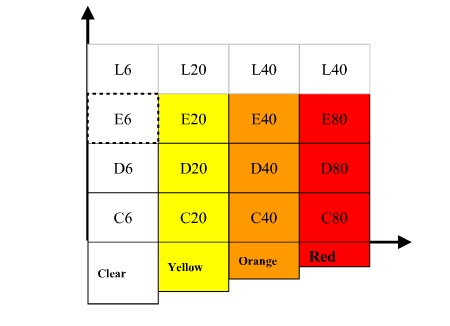
\includegraphics[scale=1]{Imagens/img-Crystal.jpg}
    \caption{Parâmetros conforme o nível crítico}
    \label{fig:crystal1}
\end{figure}

\begin{itemize}
    \item C de Confort (Conforto), casos em que a falha do sistema ocasiona a perda de credibilidade do utilizador devido a não atender este conforto.
    \item D de Discretionary Money (Dinheiro disponível para uso conforme necessário, cujo uso depende de decisão de alguém com poder de decisão). Casos em que a falha do sistema ocasiona a perda de dinheiro, mas de valor inexpressivo.
    \item E de Essencial Money (Dinheiro essencial – dinheiro indispensável, absolutamente necessário) casos em que a falha do sistema ocasiona a perda de um quantia indispensável, grandes valores.
    \item L de Life (Vida) casos em que a falha do sistema ocasiona a perda de Vidas, tendo como referência um software de piloto automático onde uma falha poderia fazer cair um avião.
\end{itemize}

\subsection{Fases do Crystal}

\begin{figure}[H]
    \centering
    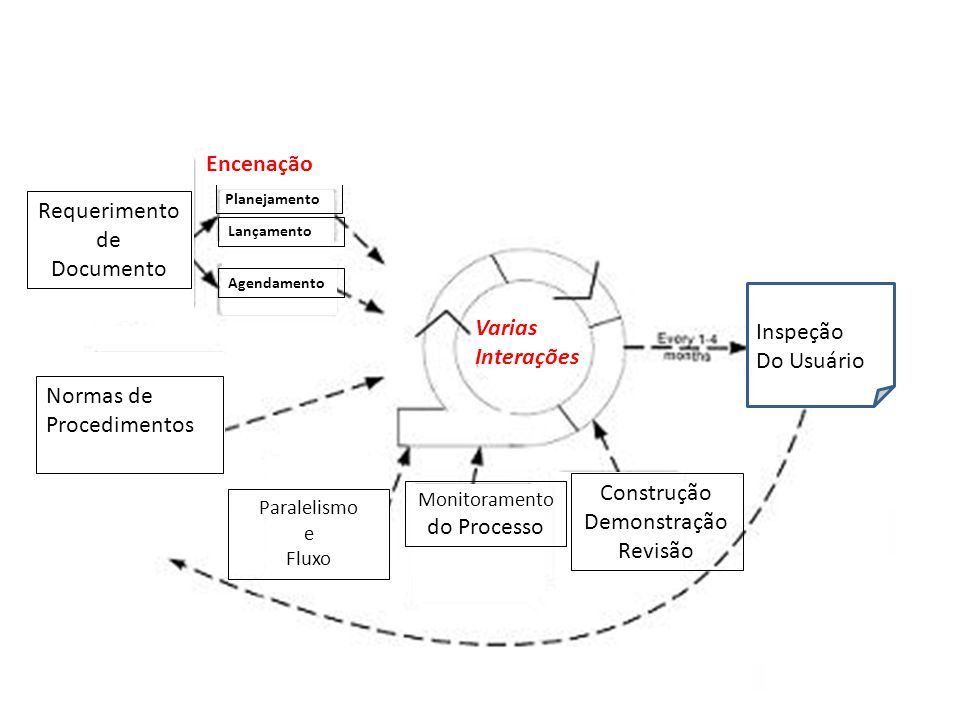
\includegraphics[scale=0.5]{Imagens/slide_1.jpg}
    \caption{Fases do Crystal}
    \label{fig:crystal2}
\end{figure}

O ciclo de vida desta família de metódos é baseado nas seguintes etapas:

\begin{itemize}

    \item Staging: Planeamento da próxima iteração do sistema. A equipa seleciona os requisitos que serão implementados na iteração e o prazo da sua entrega;
    \item Edição e revisão: Construção, demonstração e revisão dos objetivos da iteração;
    \item Monitorização: O processo é monitorizado em relação ao progresso e à estabilidade da equipa;
    \item Paralelismo e fluxo: No Crystal Orange as diferentes equipas podem operar com máximo paralelismo.
    \item Inspeção dos utilizadores: são sugeridas duas a três inspeções feitas por utilizadores a cada iteração;
    \item Workshops: são reuniões que ocorrem antes e depois de cada iteração, com o objetivo de analisar o progresso do projeto;
    \item Local matters: são os procedimentos a serem aplicados, que variam de acordo com o tipo de projeto;
    \item Work Products: sequência de lançamento, modelos de objetos comuns, manual do utilizadores, casos de teste e migração de código;
    \item Standards (padrões): padrões de notação, convenções de produto, formatação e qualidade usadas no projeto;
    \item Tools: Ferramentas mínimas utilizadas.
\end{itemize}

\subsection{Principais Conceitos}

\begin{itemize}

    \item Entregas frequentes: os proprietários de projetos-cliente podem esperar resultados da equipa a cada dois meses;
    \item Feedback contínuo: Toda a equipa do projeto reúne-se regularmente para discutir as atividades do projeto.
    \item Comunicação constante: Para pequenos projetos é esperado que toda a equipa tenha que estar na mesma sala;
    \item Segurança: O foco dos métodos Crystal nos aspetos relacionados com a segurança é algo único. 
    \item Foco: Os membros da equipa devem conhecer dois ou três itens prioritários e cada membro deve trabalhar com tempo para os concluir sem interrupção.
    \item Acesso aos utilizadores: como a maioria dos métodos ágeis, o Crystal espera que a equipa do projeto tenha acesso a um ou mais utilizadores do sistema a ser construído.
    \item Testes automatizados e Integração: o Crystal tem várias capacidades para a verificação da funcionalidade do projeto.
\end{itemize}

\newpage

\section{Test Driven Development}

O método de Test Driven Development (TDD) é um método Ágil de desenvolvimento de software que relaciona os conceitos de verificação e validação, com um ciclo curto de repetições: Em primeiro lugar o programador tem que escrever um caso de teste automatizado que define uma melhoria desejada ou uma nova funcionalidade. Só depois, é produzido o código que possa ser validado pelo teste para posteriormente o código ser refatorado para um cºodigo sobre padrões aceitáveis. O método foi desenvolvido originalmente por Kent Bec em 2003, com os princípios que esta técnica originasse e encorajasse designs de código simples e que inspirassem confiança.

\subsection{Fases do TDD}

O método TDD é, à semelhança de outros métodos, constituído por várias fases bem distintas:

\begin{figure}[H]
    \centering
    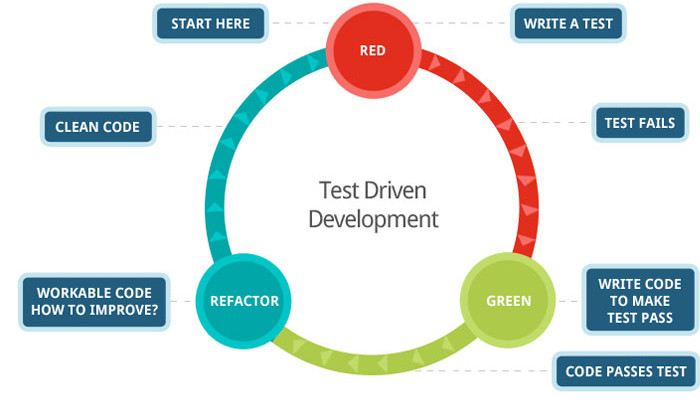
\includegraphics[scale=0.8]{Imagens/stride-nyc-test-driven-development-chart-700x400.jpg}
    \caption{Fases do TDD}
    \label{fig:tdd1}
\end{figure}


O método ASD tem, à semelhança de outros métodos, três fases: Especulação, Colaboração e Aprendizagem.

\subsubsection{Fase 1 - Adicionar um teste}

No método de Test Driven Development, cada nova funcionalidade inicia com a criação de um teste. Este teste precisa inevitavelmente de falhar porque é escrito antes da funcionalidade ser implementada. Para escrever um teste, o programador precisa de entender as especificações e requisitos da funcionalidade, à custa de casos de uso ou User Stories que cubram os requisitos e exceções condicionais. Esta é a diferenciação entre TDD e escrever testes de unidade depois do código desenvolvido, tornando o programador mais focado nos requisitos antes do código.

\subsubsection{Fase 2 - Executar todos os testes}

Esse passo valida se todos os testes criados estão a funcionar corretamente e se o novo teste não traz nenhum equívoco, sem requerer nenhum código novo. O novo teste deve então falhar pela razão esperada: a funcionalidade ainda não foi desenvolvida. Isto aumenta a confiança que se está a testar a coisa certa, e que o teste apenas irá passar nos em que deve passar.
\subsubsection{Fase 3 - Escrever código}
O próximo passo é o escrever código que irá fazer com o teste passe. O novo código escrito até esse ponto poderá não ser perfeito e pode, por exemplo, passar no teste de uma forma não elegante. Isso é aceitável porque posteriormente será refatorizado/melhorado. O importante é que o código escrito seja apenas construído para passar no teste, não devendo ser acrescentadas funcionalidades extras.
\subsubsection{Fase 4 - Executar os testes}
Se todos os testes passam, o programador pode ficar confiante de que o código possui todos os requisitos testados. Este é um bom ponto que inicia o passo final do ciclo TDD.

\subsubsection{Fase 5 - Refatorizar o código}
Neste ponto o código pode ser limpo como necessário. Ao re-executar os testes, o programador pode confiar que a refatoração não é um processo danoso a qualquer funcionalidade existente. Um conceito relevante neste momento é o de remoção da duplicação de código, considerado um importante aspeto no design de um software. Nesse caso, entretanto, isso aplica remover qualquer duplicação entre código de teste e código de produção.
\subsubsection{Fase 6 - Repetir}
Iniciado com outro teste, o ciclo é então repetido, empurrando a funcionalidade para a frente. O tamanho dos passos deve ser pequeno. Se o novo código não satisfaz rapidamente um novo teste, ou outros testes falham inesperadamente, o programador deve desfazer ou reverter. A integração contínua ajuda na criação de pontos reversíveis. É importante lembrar que ao usar bibliotecas externas não é interessante gerar iterações tão pequenas que possam efetivamente testar a biblioteca, a menos que haja alguma razão para acreditar que a biblioteca tenha defeitos ou não que seja suficientemente completa.

\subsection{Limitações do TDD}

\begin{enumerate}
    \item Desenvolvimento dirigido com testes é difícil de usar em situações onde os testes totalmente funcionais são requisitos para determinar o sucesso ou falha. Exemplos disso são interfaces gráficas, programas que trabalham com base de dados, e muitos outros que dependem de configurações específicas de rede. O TDD encoraja os programadores a incluir o mínimo de código funcional em módulos e maximizar a lógica, que é extraída no código de teste, usando Fakes mocks para representar o mundo externo.
    \item Suporte genérico é essencial. Se todas as organizações não acreditarem que TDD serve para melhorar o produto, a gestão irá considerar que o tempo gasto em testes é um desperdicio.
    \item Os próprios testes tornam-se parte da manutenção do projeto. Testes mal-escritos, por exemplo, que incluem strings de erro ou aqueles que são suscetíveis a falhas, são caros para manter. Há um risco em que testes que geram falsas falhas tenderem a serem ignorados. Assim quando uma falha real ocorre, pode não ser detetada. É possível escrever testes de baixa e fácil manutenção, por exemplo pelo re-uso das strings de erro, podendo ser o objetivo durante a fase de refatoração descrita acima.
    \item O nível de cobertura e detalhe do teste alcançado durante repetitivos ciclos de TDD não pode ser facilmente re-criado numa data tardia. Com o passar do tempo os testes vão-se tornando cada vez mais, mais preciosos. Se existe uma arquitetura pobre, um mau design ou uma estratégia de teste mal feita leva a uma mudança tardia, fazendo com que dezenas de testes falhem.
    \item Podem existir lacunas inesperadas na cobertura dos testes. Talvez um ou mais programadoresde uma equipa não foram submetidos ao uso de TDD e não escrevem testes apropriadamente, talvez muitos conjuntos de testes foram invalidados, excluídos ou desativados acidentalmente ou com o intuito de serem melhorados posteriormente. Se isto acontecer, poderá existir uma grande quantidade de testes que serão corrigidos tardiamente e a sua refactoração será mal feita, 
    \item Os testes são criados num ambiente de desenvolvimento por um programador, que posteriormente irá também escrever o código para passar nesse teste. Os testes podem, por isso, conter os mesmos "pontos cegos" do que o código. 
    \item O alto número de testes pode trazer uma falsa sensação de segurança, resultando num menor nível de atividade da garantia de qualidade, como testes de integração e aceitação.
\end{enumerate}
\chapter{Comparação entre Métodos}
\label{cht:grupos}

Anteriormente foi feito um estudo sobre os métodos Ágil mais usados hoje em dia. No entanto, é necessário comparar os vários métodos por forma a podermos tirar conclusões e enquadrar estes métodos nos vários quadrantes, segundo as características próprias de cada um.
É normal não usar a mesma abordagem para um projeto onde é necessário criar apenas uma página web ou uma peça de software para um satélite da NASA. É também normal não usar a mesma abordagem com uma equipa de seis pessoas, do que com uma de sessenta pessoas ou até mesmo seiscentas pessoas. Diferentes situações exigem abordagens diferentes.
É fácil entender que é necessário alinhar a nossa abordagem mediante as variáveis do projeto em questão, e é por isso necessário não só dividir os vários métodos (tradicionais e Ágil) em várias categorias. 

\subsection{A necessidade de flexibilidade}

Para se ser bem sucedido no desenvolvimento de um software é necessário ser flexível na escolha do método utilizado. Existindo várias razões pelas quais é importante fazer:

\begin{itemize}
    \item \textbf{Diferentes tecnologias requerem diferentes técnicas} - Por exemplo, métodos orientados a objetos servem melhor projetos que usam tecnologias orientadas a objetos e métodos orientados aos dados servem melhor aplicações orientadas aos dados.
    \item \textbf{Cada pessoa é única} - Cada constituinte da equipa tem um background diferente, preferências de trabalho diferentes e diferentes gostos. Um método que sirva bem uma equipa, pode não resultar bem noutra equipa.
    \item \textbf{Cada equipa é única} - As equipas são feitas por pessoas, e como as pessoas são únicas a união destas pessoas torna-se também única. É importante adaptar o método de trabalho à equipa.
    \item \textbf{As necessidades exteriores podem variar} - Por exemplo, um projeto pode estar sujeito a regulamentações governamentais, ou pode estar sujeito a restrições de fornecedores ou até mesmo a desenvolvimento de terceiros. É importante também adaptar o método de trabalho para incorporar fatores exteriores.
    \item \textbf{As categorias dos projetos variam} - Diferentes tipos de projetos requerem diferentes abordagens porque cada categoria tem as suas prioridades e objetivos.
    \item \textbf{As categorias dos métodos variam} - Cada método Ágil tem as suas vantagens e desvantagens.
\end{itemize}

\subsection{As categorias dos métodos}

Os métodos de desenvolvimento podem ser separados em quatro categorias distintas:

\begin{itemize}
    \item \textbf{Code and Fix} - Abordagem conhecida também como "hacking". É por norma uma abordagem caótica e muitas vezes não planeada, ou quando planeada o plano é rapidamente abandonado. As estimativas e cronogramas, quando feitos, raramente são cumpridos na prática.
    \item \textbf{Rigoroso} - Os projetos de software nesta categoria são bem definidos e geralmente incluem procedimentos detalhados que os programadores devem seguir com bastante rigor. Por exemplo, os requisitos são identificados, revistos e aceites. O design do sistema é feito, revisto e aceite. Há espaço para feedback entre as fases, embora esse feedback seja fornecido por meio de um procedimento bem estruturado e as alterações revistas e aceites. Os sistemas são entregues de forma incremental.
    \item \textbf{Iterativo Rigoroso} - Os processos de software nesta categoria são bem definidos e geralmente incluem procedimentos detalhados que os programadores devem aplicar de maneira iterativa. Por exemplo, os requisitos do projeto podem ser definidos inicialmente em alto nível, com os detalhes posteriormente detalhados conforme necessário. O software é entregue numa base incremental após curtos ciclos de lançamento.
    \item \textbf{Ágil} - Abordagem para o desenvolvimento de software orientada para pessoas, que permite que respondam efetivamente às mudanças e que resulta na criação de sistemas de trabalho que atendam às necessidades dos stakeholders. Os processos de software nesta categoria são definidos a alto nível, geralmente apresentados como uma coleção de práticas ou filosofias. Os principais métodos Ágil foram já identificados e descritos no capítulo anterior.
\end{itemize}

Cada categoria apela a uma mentalidade diferente. Por exemplo, os métodos Code and Fix são mais apropriados para programadores independentes. Os métodos Rigorosos são apropriados para equipas que querem ter uma abordagem inicial simples, geralmente em indústrias muito regulamentadas e burocráticas. Os métodos Rigorosos Iterativos funcionam bem em ambientes que são propensos a burocracia, mas com abertura suficiente para práticas arriscadas promovidas pelo desenvolvimento iterativo. Por fim, os métodos Ágil são uma abordagem nova e que normalmente permite ter em conta todos os stakeholders do projeto.

\subsection{Comparação entre métodos}

No gráfico em baixo poderemos ver a comparação entre os vários métodos, tendo em conta a adaptação a cada projeto (de ad-hoc a prescriptive) e o tamanho do ciclo do projeto (de full lifecycle a partial methodology), ou seja, se acompanha toda a vida do projeto ou se será necessário adotar um novo método mais tarde. 

\begin{figure}[H]
    \centering
    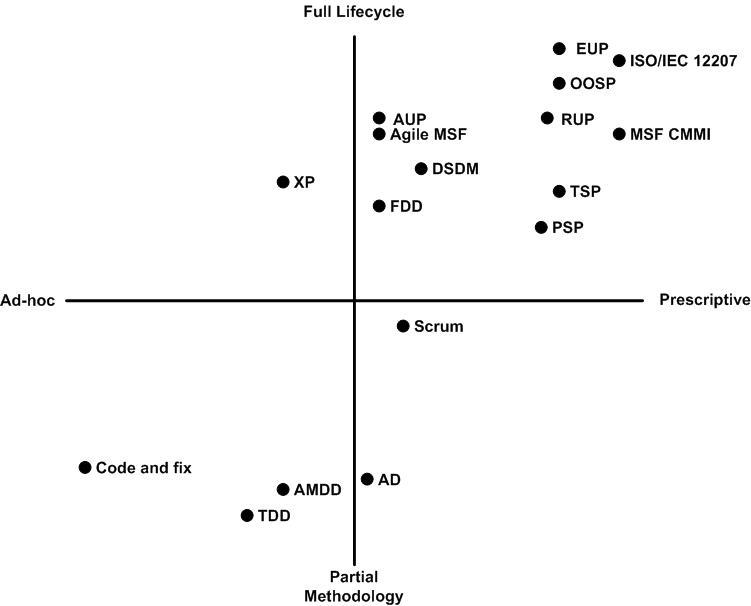
\includegraphics[scale=0.5]{Imagens/processComparisons.jpg}
    \caption{Comparação dos vários métodos}
    \label{fig:compme}
\end{figure}


\subsection{A necessidade de usar mais do que um método}

Nesta comparação foram tidos em conta os vários métodos, mais tradicionais ou mais inovadores, já que nem todas as organizações estão pré-dispostas e têm as características necessárias para adotar uma metodologia Ágil na sua organização interna. O facto de termos tido em conta também os métodos mais tradicionais deve-se ao facto de os métodos Ágil não servirem tudo, nem serem apropriados para tudo, especialmente quando os projetos de software podem variar tanto. É necessário por isso ter uma mente aberta e escolher o método mais apropriado. Nos capítulos seguintes tenta-se criar um método de diagnóstico para ser usado no início do projeto com o objetivo de tirar conclusões iniciais sobre a utilização ou não de um método Ágil.
\\É possível, numa mesma organização, adotar e suportar vários métodos dos descritos anteriormente, tendo, no entanto, em conta o seguinte:

\begin{enumerate}
    \item Não variar muito a quantidade de métodos e aplicar apenas um pequeno conjunto que sirvam a grande maioria dos projetos desenvolvidos.
    \item Não basta adotar o método, terá que haver um esforço inicial de trabalhar e modificar o método para se moldar à equipa que o vai usar.
    \item Definir objetivos em comum a todos os projetos, não procedimentos porque como já foi dito, cada projeto é um projeto.
    \item Definir bem a terminologia utilizada.
    \item Ser flexível.
    \item Priorizar requisitos e objetivos.
\end{enumerate}

De seguida apresenta-se uma tabela com as principais características dos métodos Ágil e que pode ser utilizada como ponto de partida para a escolha.

\begin{sidewaystable}[ht]
\centering
\label{grupos}
\resizebox{\textwidth}{!}{
\begin{tabular}{|l|l|l|l|l|l|l|}
\hline
Características/Método         & Extreme Programming                                                                                               & Scrum                                                               & Dynamic Systems Development Method                        & Test Driven Development                                                       & Adaptive Software Development                                                                         & Crystal Methods                                                           \\ \hline
Abordagem                      & Incrementos iterativos                                                                                            & Incrementos iterativos                                              & Iterativo                                                 & Iterativo                                                                     & Iterativo                                                                                             & Incremental                                                               \\ \hline
Tempo recomendado por iteração & Entre 1 e 6 semanas                                                                                               & Entre 2 a 4 semanas                                                 & 80\% da solução em 20\% do tempo total                    & Entre 2 dias e 2 semanas                                                      & Entre 4 e 8 semanas                                                                                   & Depende do método da família                                              \\ \hline
Equipa                         & Equipas pequenas (\textless{}20 pessoas)                                                                          & Aplicável a equipas de todos os tamanhos                            & Todos os tamanhos, equipa independente                    & Mais de uma equipa                                                            & Equipas pequenas (entre 5 a 9 membros)                                                                & Todos tamanho, depende do método da família                               \\ \hline
Comunicação da equipa          & Informal com reuniões diárias                                                                                     & Informal com reuniões diárias                                       & Baseado em documentação                                   & Baseado em documentação                                                       & Informal e pessoal                                                                                    & Informal e pessoal                                                        \\ \hline
Tamanho do Projeto             & Projetos pequenos                                                                                                 & Todos os tipos projetos                                             & Todos os tipos de projetos                                & Projetos complexos e com várias funcionalidades                               & Projetos pequenos                                                                                     & Todos os tipos de projeto                                                 \\ \hline
Envolvimento do cliente        & Envolvimento total do cliente                                                                                     & O próprio clientes faz parte da equipa                              & O cliente está presente no momento dos lançamentos        & O cliente recebe relatórios                                                   & O cliente está presente no momento dos lançamentos                                                    & O cliente está presente a cada incremento                                 \\ \hline
Documentação do projeto        & Documentação básico                                                                                               & Documentação básica                                                 & Documentação básica                                       & Documentação é importante                                                     & Documentação básica                                                                                   & Documentação básica                                                       \\ \hline
Especialidades                 & Testes, User Stories, Refatoração                                                                                 & Sprint, Sprint backlog, Scrum master                                & Prototipagem                                              & Diagramas UML                                                                 & Ciclo de aprendizagem                                                                                 & Vários métodos dentro da família adaptáveis a qualquer situação e projeto \\ \hline
Vantagens                      & Ambiente de trabalho aberto em que o cliente pode ser parte da equipa, práticas bem definidas, Feedback constante & Alto nível de comunicação e colaboração                             & Os requisitos são prioridade, gestão do projeto eficiente & Os relatórios e a documentação permitem efetuar várias tarefas ao mesmo tempo & É importante desenvolver os componentes de maior risco primeiro, o ciclo de aprendizagem é importante & A metodologia ajusta-se ao tipo de projeto e tamanho da equipa            \\ \hline
Desvantagens                   & Pouca documentação, pouca disciplina, a presença do cliente pode ser crucial                                      & Pouca documentação, o controlo sobre o projeto é por vezes reduzido & Documentação complexa                                     & Podem existir "pontos cegos"                                                  & Pouca documentação                                                                                    & A coordenação pode ser pouco eficiente entre as equipas                   \\ \hline
\end{tabular}}
\end{sidewaystable}
\chapter{Desenvolvimento da Metodologia de Diagnóstico}
\label{cht:projetoagil}

Depois da recolha e estudo do panorama das Metodologias Ágil é possível adquirir uma série de características em comum entre elas e que nos permitem distinguir de maneira eficaz das metodologias mais tradicionais como é o caso dos Modelos em Cascata.
\\A questão de quando se deve, ou não usar a Metodologia Ágil num determinado projeto depende de inúmeros fatores, incluindo fatores como o número de recursos disponíveis, o tipo de projeto de desenvolvimento, a especialização da equipa, etc.
\\
\\Apesar da sua popularidade, especialmente na indústria do software e as muitas vantagens que traz relativamente às metodologias mais tradicionais, a Metodologia Ágil não deve ser usada em todos os projetos. Antes de partir para qualquer tipo de desenvolvimento do produto em questão deve ser realizado um planeamento completo para entender se os recursos são suficientes, se a equipa está adaptada e se há uma necessidade real de usar este conjunto de práticas de desenvolvimento. Não se deve usar a metodologia Ágil apenas por uma questão de moda, porque a metodologia sozinha nunca levará um projeto ao sucesso.
\vspace{10mm}

\begin{figure}[H]
    \centering
    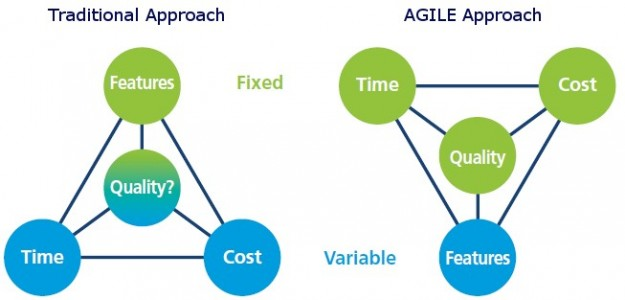
\includegraphics[scale=0.7]{Imagens/Traditional-Vs-Agile-e1409736279325.jpg}
    \caption{Comparação entre os Métodos Tradicionais e Métodos Ágeis}
    \label{fig:compta}
\end{figure}


\newpage

\subsection{Metodologia de Diagnóstico}

\begin{framed}
\noindent\textbf{Metodologia de Diagnóstico de um Projeto Ágil}
\qquad
Versão 1.0
\vspace{2mm}
\newline Este método de diagnóstico deve ser usado na fase de pré-planeamento de um projeto e servirá como uma escolha inicial entre os métodos mais tradicionais e um método Ágil. A primeira versão deste questionário apenas serve para indicar se deve ou não ser usada uma Metodologia Ágil, o método Ágil em específico não é tido em conta.
\vspace{1mm}
\newline Este questionário é constituído por 12 perguntas. As perguntas podem ter cotação 1, 2 ou 3 o que mede a sua importância e serve como fator multiplicativo.
\vspace{5mm}
\newline\textbf{Questão 1 - } Há uma necessidade dentro da sua organização de mudar de método de desenvolvimento?
\newline \begin{center} Sim \hspace{30mm} Não \end{center}
\vspace{2mm}
\newline\textbf{Questão 2 - } O projeto tem urgência e os prazos para sua conclusão são apertados?
\newline \begin{center} Sim \hspace{30mm} Não\end{center}
\vspace{2mm}
\newline\textbf{Questão 3 - } A sua equipa é bastante organizada?
\newline \begin{center} Sim \hspace{30mm} Não \end{center}
\vspace{2mm}
\newline\textbf{Questão 4 - } O cliente necessita de documentação clara de cada ciclo de desenvolvimento?
\newline \begin{center} Sim \hspace{30mm} Não \end{center}
\vspace{2mm}
\newline\textbf{Questão 5 - } O cliente necessita de aprovar o projeto a cada fase de desenvolvimento?
\newline \begin{center} Sim \hspace{30mm} Não \end{center}
\vspace{2mm}
\newline\textbf{Questão 6 - } O cliente está mais habituado e prefere usar métodos de desenvolvimento mais tradicionais?
\newline \begin{center} Sim  \hspace{30mm} Não\end{center}
\newline\textbf{Questão 7 - } Na sua perspetiva e mediante os projetos que a sua organização costuma trabalhar, qual é o tamanho do projeto?
\newline \begin{center} Pequeno \hspace{17mm} Médio\hspace{17mm}Grande\end{center}
\vspace{2mm}
\newline\textbf{Questão 8 - } São necessárias múltiplas variantes do projeto, ou pelo menos, são desejáveis?
\newline \begin{center} Sim\hspace{30mm} Não\end{center}
\vspace{2mm}
\newline\textbf{Questão 9 - } Qual é a área do projeto?
\newline \begin{center} Software ou Hardware \hspace{17mm} Serviços Financeiros \hspace{17mm}Serviços Profissionais \hspace{17mm} Outros\end{center}
\vspace{2mm}
\newline\textbf{Questão 10 - } O projeto está bem documentado e todos os requisitos estão definidos à partida?
\newline \begin{center} Sim \hspace{30mm} Não\end{center}
\vspace{2mm}
\newline\textbf{Questão 11 - } O cliente terá uma participação ativa no desenvolvimento do produto?
\newline \begin{center} Sim \hspace{30mm} Não \end{center}
\vspace{2mm}
\newline\textbf{Questão 12 - } Os elementos da sua equipa são pró-ativos e demonstram iniciativa?
\newline \begin{center} Sim \hspace{30mm} Não\end{center}
\vspace{10mm}

\vspace{10mm}
\begin{center}
\begin{itemize}
    \item \textbf{Menos de 10 pontos} - Os Métodos Ágil \\não são, à partida, apropriados ao seu projeto.
    \item \textbf{Entre 10 e 15 pontos} - Os Métodos Ágil talvez \\sejam apropriados mas necessita de uma segunda opinião.
    \item \textbf{Mais de 15 pontos} - Os Métodos Ágil são\\ apropriados ao seu projeto.
\end{itemize}
\end{center}
\end{framed}

\begin{table}[]
\centering
\label{my-label}
\begin{tabular}{|l|l|l|l|l|}
\hline
Pergunta/Pontuação & 0 pontos & 1 ponto                                                              & 2 pontos                                                           & 3 pontos                                                           \\ \hline
Pergunta 1         & Não      & Sim                                                                  & -                                                                  & -                                                                  \\ \hline
Pergunta 2         & Não      & -                                                                    & Sim                                                                & -                                                                  \\ \hline
Pergunta 3         & Não      & Sim                                                                  & -                                                                  & -                                                                  \\ \hline
Pergunta 4         & Sim      & -                                                                    & Não                                                                & -                                                                  \\ \hline
Pergunta 5         & Sim      & Não                                                                  & -                                                                  & -                                                                  \\ \hline
Pergunta 6         & Sim      & -                                                                    & Não                                                                & -                                                                  \\ \hline
Pergunta 7         & Grande   & Médio                                                                & Pequeno                                                            & -                                                                  \\ \hline
Pergunta 8         & Não      & Sim                                                                  & -                                                                  & -                                                                  \\ \hline
Pergunta 9         & Outros   & \begin{tabular}[c]{@{}l@{}}Serviços \\ \\ Profissionais\end{tabular} & \begin{tabular}[c]{@{}l@{}}Serviços \\ \\ Financeiros\end{tabular} & \begin{tabular}[c]{@{}l@{}}Software ou \\ \\ Hardware\end{tabular} \\ \hline
Pergunta 10        & Sim      & -                                                                    & Não                                                                & -                                                                  \\ \hline
Pergunta 11        & Não      & Sim                                                                  & -                                                                  & -                                                                  \\ \hline
Pergunta 12        & Não      & Sim                                                                  & -                                                                  & -                                                                  \\ \hline
\end{tabular}
\end{table}

\chapter{Aplicação do Método}
\label{cht:aplicacao}

Neste capítulo é aplicado a metodologia desenvolvida nos capítulos anteriores a dois projetos, como forma de demonstração e validação do que foi desenvolvido.
\\O primeiro projeto é um projeto desenvolvido no contexto académico e o segundo é um projeto de uma empresa.

\vspace{5mm}

\subsection{Projeto académico}

O projeto foi proposto aos alunos do Mestrado em Engenharia Informática na unidade curricular de Engenharia Web. Em grupos de no máximo 4 elementos, os alunos devem desenvolver com tecnologias Web uma plataforma de trading. O prazo de entrega é o dia 14 de junho, sendo que existe uma entrega intermédia dia 10 de maio, o que dá cerca de 4 meses para desenvolver todo o projeto. É necessário desenvolver tanto o frontend da aplicação como o backend, o projeto tem cerca de 8 requisitos obrigatórios.

\begin{framed}
\noindent\textbf{Metodologia de Diagnóstico de um Projeto Ágil}
\qquad
Versão 1.0
\vspace{2mm}
\newline Este método de diagnóstico deve ser usado na fase de pré-planeamento de um projeto e servirá como uma escolha inicial entre os métodos mais tradicionais e um método Ágil. A primeira versão deste questionário apenas serve para indicar se deve ou não ser usada uma Metodologia Ágil, o método Ágil em específico não é tido em conta.
\vspace{1mm}
\newline Este questionário é constituído por 12 perguntas. As perguntas podem ter cotação 1, 2 ou 3 o que mede a sua importância e serve como fator multiplicativo.
\vspace{5mm}
\newline\textbf{Questão 1 - } Há uma necessidade dentro da sua organização de mudar de método de desenvolvimento?
\newline \begin{center} Sim (1 ponto) \hspace{30mm} \textbf{Não (0 pontos)}\end{center}
\vspace{2mm}
\newline\textbf{Questão 2 - } O projeto tem urgência e os prazos para sua conclusão são apertados?
\newline \begin{center} \textbf{Sim (2 pontos)} \hspace{30mm} Não (0 pontos)\end{center}
\vspace{2mm}
\newline\textbf{Questão 3 - } A sua equipa é bastante organizada?
\newline \begin{center} Sim (1 ponto) \hspace{30mm} \textbf{Não (0 pontos)}\end{center}
\vspace{2mm}
\newline\textbf{Questão 4 - } O cliente necessita de documentação clara de cada ciclo de desenvolvimento?
\newline \begin{center} Sim (0 pontos) \hspace{30mm} \textbf{Não (2 pontos)}\end{center}
\vspace{2mm}
\newline\textbf{Questão 5 - } O cliente necessita de aprovar o projeto a cada fase de desenvolvimento?
\newline \begin{center} \textbf{Sim (0 pontos)} \hspace{30mm} Não (1 ponto)\end{center}
\vspace{2mm}
\newline\textbf{Questão 6 - } O cliente está mais habituado e prefere usar métodos de desenvolvimento mais tradicionais?
\newline \begin{center} Sim (0 pontos) \hspace{30mm} \textbf{Não (2 pontos)}\end{center}
\newline\textbf{Questão 7 - } Na sua perspetiva e mediante os projetos que a sua organização costuma trabalhar, qual é o tamanho do projeto?
\newline \begin{center} Pequeno (2 pontos) \hspace{17mm} \textbf{Médio (1 ponto)}\hspace{17mm}Grande (0 pontos)\end{center}
\vspace{2mm}
\newline\textbf{Questão 8 - } São necessárias múltiplas variantes do projeto, ou pelo menos, são desejáveis?
\newline \begin{center} Sim (1 ponto) \hspace{30mm} \textbf{Não (0 pontos)}\end{center}
\vspace{2mm}
\newline\textbf{Questão 9 - } Qual é a área do projeto?
\newline \begin{center} \textbf{Software ou Hardware (3 pontos)}\hspace{17mm} Serviços Financeiros (2 pontos)\hspace{17mm}Serviços Profissionais (1 ponto)\hspace{17mm} Outros (0 pontos)\end{center}
\vspace{2mm}
\newline\textbf{Questão 10 - } O projeto está bem documentado e todos os requisitos estão definidos à partida?
\newline \begin{center} \textbf{Sim (0 pontos)} \hspace{30mm} Não (2 pontos)\end{center}
\vspace{2mm}
\newline\textbf{Questão 11 - } O cliente terá uma participação ativa no desenvolvimento do produto?
\newline \begin{center} Sim (1 ponto) \hspace{30mm} \textbf{Não (0 pontos)}\end{center}
\vspace{2mm}
\newline\textbf{Questão 12 - } Os elementos da sua equipa são pró-ativos e demonstram iniciativa?
\newline \begin{center}\textbf{Sim (1 ponto)} \hspace{30mm} Não (0 pontos)\end{center}

\vspace{10mm}
\begin{center}
\begin{itemize}
    \item \textbf{Menos de 10 pontos} - Os Métodos Ágil \\não são, à partida, apropriados ao seu projeto.
    \item \textbf{Entre 10 e 15 pontos} - Os Métodos Ágil talvez \\sejam apropriados mas necessita de uma segunda opinião.
    \item \textbf{Mais de 15 pontos} - Os Métodos Ágil são\\ apropriados ao seu projeto.
\end{itemize}
\end{center}
\end{framed}

O total de pontos obtidos é \textbf{11 pontos}. Por isto, o projeto fica no patamar intermédio. É por isso necessário uma segunda opinião, ou pelo menos, uma reflexão mais profunda e a longo prazo se é vantajoso usar os Métodos Ágeis.

\newpage

\subsection{Projeto empresarial - Aplicação para supermercado}

O projeto a ser desenvolvido tem como finalidade o desenvolvimento de uma aplicação mobile para uma conhecida marca de supermercados. Esta aplicação deverá ser capaz de receber pedidos de compras dos clientes a partir de uma listagem de todos os produtos em loja. A  equipa de desenvolvimento vai ser constituída por 8 elementos, entre designers, direção e programadores. O prazo para a conclusão e entrega final da aplicação é o dia 21 de junho, o que desde o pedido inicial até à entrega final dá cerca de 6 meses de trabalho. O cliente apenas fez o pedido inicial, mas não definiu os requisitos totalmente, estes serão definidos à medida que o desenvolvimento vai acontecendo. É necessário uma aplicação para iOS e outra para Android.

\begin{framed}
\noindent\textbf{Metodologia de Diagnóstico de um Projeto Ágil}
\qquad
Versão 1.0
\vspace{2mm}
\newline Este método de diagnóstico deve ser usado na fase de pré-planeamento de um projeto e servirá como uma escolha inicial entre os métodos mais tradicionais e um método Ágil. A primeira versão deste questionário apenas serve para indicar se deve ou não ser usada uma Metodologia Ágil, o método Ágil em específico não é tido em conta.
\vspace{1mm}
\newline Este questionário é constituído por 12 perguntas. As perguntas podem ter cotação 1, 2 ou 3 o que mede a sua importância e serve como fator multiplicativo.
\vspace{5mm}
\newline\textbf{Questão 1 - } Há uma necessidade dentro da sua organização de mudar de método de desenvolvimento?
\newline \begin{center} Sim (1 ponto) \hspace{30mm} \textbf{Não (0 pontos)}\end{center}
\vspace{2mm}
\newline\textbf{Questão 2 - } O projeto tem urgência e os prazos para sua conclusão são apertados?
\newline \begin{center} \textbf{Sim (2 pontos)} \hspace{30mm} Não (0 pontos)\end{center}
\vspace{2mm}
\newline\textbf{Questão 3 - } A sua equipa é bastante organizada?
\newline \begin{center} \textbf{Sim (1 ponto)} \hspace{30mm} Não (0 pontos)\end{center}
\vspace{2mm}
\newline\textbf{Questão 4 - } O cliente necessita de documentação clara de cada ciclo de desenvolvimento?
\newline \begin{center} Sim (0 pontos) \hspace{30mm} \textbf{Não (2 pontos)}\end{center}
\vspace{2mm}
\newline\textbf{Questão 5 - } O cliente necessita de aprovar o projeto a cada fase de desenvolvimento?
\newline \begin{center} \textbf{Sim (0 pontos)} \hspace{30mm} Não (1 ponto)\end{center}
\vspace{2mm}
\newline\textbf{Questão 6 - } O cliente está mais habituado e prefere usar métodos de desenvolvimento mais tradicionais?
\newline \begin{center} Sim (0 pontos) \hspace{30mm} \textbf{Não (2 pontos)}\end{center}
\newline\textbf{Questão 7 - } Na sua perspetiva e mediante os projetos que a sua organização costuma trabalhar, qual é o tamanho do projeto?
\newline \begin{center} Pequeno (2 pontos) \hspace{17mm} \textbf{Médio (1 ponto)}\hspace{17mm}Grande (0 pontos)\end{center}
\vspace{2mm}
\newline\textbf{Questão 8 - } São necessárias múltiplas variantes do projeto, ou pelo menos, são desejáveis?
\newline \begin{center} \textbf{Sim (1 ponto)} \hspace{30mm} Não (0 pontos)\end{center}
\vspace{2mm}
\newline\textbf{Questão 9 - } Qual é a área do projeto?
\newline \begin{center} \textbf{Software ou Hardware (3 pontos)}\hspace{17mm} Serviços Financeiros (2 pontos)\hspace{17mm}Serviços Profissionais (1 ponto)\hspace{17mm} Outros (0 pontos)\end{center}
\vspace{2mm}
\newline\textbf{Questão 10 - } O projeto está bem documentado e todos os requisitos estão definidos à partida?
\newline \begin{center} Sim (0 pontos) \hspace{30mm} \textbf{Não (2 pontos)}\end{center}
\vspace{2mm}
\newline\textbf{Questão 11 - } O cliente terá uma participação ativa no desenvolvimento do produto?
\newline \begin{center} \textbf{Sim (1 ponto)} \hspace{30mm} Não (0 pontos)\end{center}
\vspace{2mm}
\newline\textbf{Questão 12 - } Os elementos da sua equipa são pró-ativos e demonstram iniciativa?
\newline \begin{center} \textbf{Sim (1 ponto)} \hspace{30mm} Não (0 pontos)\end{center}

\vspace{10mm}
\begin{center}
\begin{itemize}
    \item \textbf{Menos de 10 pontos} - Os Métodos Ágil \\não são, à partida, apropriados ao seu projeto.
    \item \textbf{Entre 10 e 15 pontos} - Os Métodos Ágil talvez \\sejam apropriados mas necessita de uma segunda opinião.
    \item \textbf{Mais de 15 pontos} - Os Métodos Ágil são\\ apropriados ao seu projeto.
\end{itemize}
\end{center}
\end{framed}

O total de pontos obtidos é \textbf{17 pontos}. Por isto, o projeto fica no patamar máximo. O projeto deverá sem dúvida usar uma metodologia Ágil já que se adapta às principais características deste tipo de método.
\chapter{Conclusão e Trabalho Futuro}
\label{chp:conclusao}

Depois de analisados e descritos os princípios e algumas metodologias Ágeis, constata-se que estas trouxeram melhorias notórias nos processos e fluxos de trabalho das empresas, que se convertem em maior organização, capacidade de produção e consequentemente, satisfação dos clientes. É de notar também que, apesar do que muitas pessoas possam imaginar, estas metodologias não são propriamente recentes. Já foram inventadas há alguns anos, mas só começaram a popularizar-se na área da produção de Software há relativamente pouco tempo e o seu uso tem vindo a tornar-se cada vez mais comum. Apesar das vantagens das abordagens mais Ágeis, elas têm vantagens e desvantagens e não servem para todo o tipo de projeto.\\
Na nossa opinião o método desenvolvido tem algumas características que à partida definimos como prioritárias: é simples, não demora muito a responder, é direto e ajuda a ter uma primeira perceção do método de trabalho a seguir.\\
É também importante definir que esta é apenas uma primeira versão do método de diagnóstico, será esperado que como trabalho futuro se sugira uma segunda parte do questionário que apenas seja respondida se a primeira parte indicar que o projeto deva seguir uma abordagem ágil, e onde se consiga perceber em específico que método Ágil o projeto deve seguir. Para além disso, e devido ao facto de o desenvolvimento deste projeto ter sido feito num contexto académico com prazos limitados, é também importante validar as questões num contexto real em projetos já desenvolvidos e onde se consiga ter uma perceção se as abordagens ágeis ou tradicionais resultaram.

\bibliographystyle{plain}
\bibliography{Bibliografia}

\end{document}